\documentclass{standalone}
\usepackage{pgfplots}
\usetikzlibrary{arrows.meta} 
\pgfplotsset{compat=1.18}
\begin{document}
	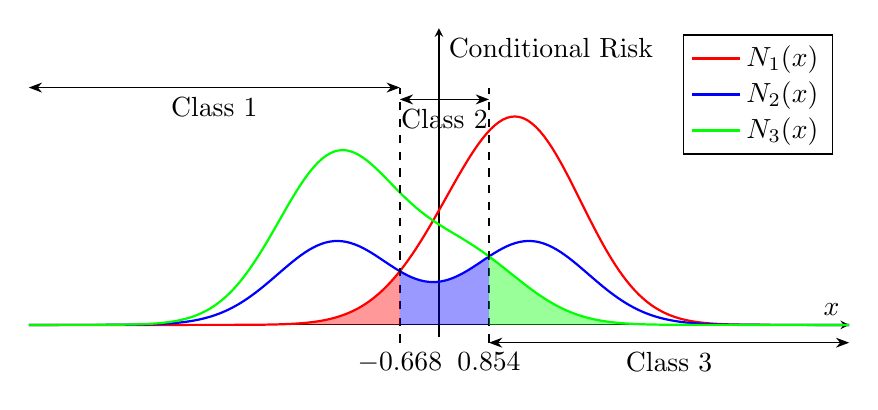
\begin{tikzpicture}
		\begin{axis}[
			domain=-7:7,
			samples=200,
			axis lines=middle,
			xlabel={$x$},			
			ylabel=Conditional Risk,
			xtick=\empty,
			ytick=\empty,
			ymin=-0.02, ymax=0.5,
			enlargelimits=false,
			clip=false,
			grid=major,
			width=12cm, height=5.5cm
			]
			\def\ua{-1.75}
			\def\ub{0.4}
			\def\uc{1.55}
			\def\sa{1}
			\def\sb{1}
			\def\sc{1}
			\def\xa{-0.668}
			\def\xb{0.854}
			
			% Normal mixture curves
			\addplot[red, thick]
			{5/17 * 1/(sqrt(2*pi*\sb)) * exp(-((x-\ub)^2)/(2*\sb))
				+ 12/17 * 1/(sqrt(2*pi*\sc)) * exp(-((x-\uc)^2)/(2*\sc))};
			\addlegendentry{$N_1(x)$}
			
			\addplot[blue, thick]
			{6/17*1/(sqrt(2*pi*\sa)) * exp(-((x-\ua)^2)/(2*\sa))
				+6/17*1/(sqrt(2*pi*\sc)) * exp(-((x-\uc)^2)/(2*\sc))};
			\addlegendentry{$N_2(x)$}
			
			\addplot[green, thick]
			{12/17*1/(sqrt(2*pi*\sa)) * exp(-((x-\ua)^2)/(2*\sa))
				+5/17*1/(sqrt(2*pi*\sb)) * exp(-((x-\ub)^2)/(2*\sb))};
			\addlegendentry{$N_3(x)$}
			
			% vertical dashed decision boundaries
			\addplot[black, dashed, thick] coordinates {(\xa,-0.03) (\xa,0.4)};
			\node[below] at (axis cs:\xa,-0.03) {$\xa$};
			
			\addplot[black, dashed, thick] coordinates {(\xb,-0.03) (\xb,0.4)};
			\node[below] at (axis cs:\xb,-0.03) {$\xb$};
			
			% Fills with corrected domain and variable
			\fill [red, opacity = .4, domain=-7:\xa, variable=\x]
			(-7, 0)
			-- plot ({\x}, {5/17 * 1/(sqrt(2*pi*\sb)) * exp(-((\x-\ub)^2)/(2*\sb))
				+ 12/17 * 1/(sqrt(2*pi*\sc)) * exp(-((\x-\uc)^2)/(2*\sc))})
			-- (\xa, 0)
			-- cycle;
			
			\fill [blue, opacity = .4, domain=\xa:\xb, variable=\x]
			(\xa, 0)
			-- plot ({\x}, {6/17*1/(sqrt(2*pi*\sa)) * exp(-((\x-\ua)^2)/(2*\sa))
				+6/17*1/(sqrt(2*pi*\sc)) * exp(-((\x-\uc)^2)/(2*\sc))})
			-- (\xb, 0)
			-- cycle;
			
			\fill [green, opacity = .4, domain=\xb:7, variable=\x]
			(\xb, 0)
			-- plot ({\x}, {12/17*1/(sqrt(2*pi*\sa)) * exp(-((\x-\ua)^2)/(2*\sa))
				+5/17*1/(sqrt(2*pi*\sb)) * exp(-((\x-\ub)^2)/(2*\sb))})
			-- (7, 0)
			-- cycle;
			
			% Labels
			\draw[Stealth-Stealth] (\xa,0.4) -- (-7,0.4)
			node[midway, below] {Class 1};
			
			\draw[Stealth-Stealth] (\xa,0.38) -- (\xb,0.38)
			node[midway, below] {Class 2};
			
			\draw[Stealth-Stealth] (7,-0.03) -- (\xb,-0.03)
			node[midway, below] {Class 3};
			
		\end{axis}
	\end{tikzpicture}
\end{document}
